\documentclass[twocolumn]{aastex631}

\usepackage{amsmath}
\usepackage{multirow}
\usepackage{natbib}
\usepackage{graphicx} 
\usepackage{aas_macros}


\begin{document}

\title{Predicting Halo Assembly Bias from Merger Tree Morphology using Graph Neural Networks and Topological Data Analysis: A Feasibility Study}

\author{AstroPilot}
\affiliation{Anthropic, Gemini \& OpenAI servers. Planet Earth.}

\begin{abstract}
We investigate the relationship between dark matter halo merger tree morphology and halo assembly bias, a key challenge in cosmology, by exploring the feasibility of using Graph Neural Networks (GNNs) to predict an assembly bias proxy from the structural properties of halo merger trees. The original intention was to use Topological Data Analysis (TDA) to guide the GNN architecture and training. Merger trees from cosmological N-body simulations were preprocessed, extracting node features (halo mass, concentration, maximum circular velocity, scale factor) and edge features (merger mass ratio, time difference). However, significant issues arose during the calculation of an assembly bias proxy, resulting in a drastic reduction of the dataset size from 1000 to only 25 merger trees, precluding the TDA component. A Graph Convolutional Network (GCN) was trained on this limited dataset to predict the assembly bias proxy. The GNN model failed to demonstrate any meaningful predictive capability, achieving a high Mean Squared Error and a large negative R-squared score on the test set. These results highlight the critical importance of sufficient data for training complex machine learning models and the challenges associated with reliably extracting assembly bias information from merger trees. While the initial attempt was unsuccessful due to data limitations, the proposed methodology warrants further investigation with larger, more robust datasets and the incorporation of TDA to quantify merger tree morphology.
\end{abstract}

\keywords{Black hole physics, Nebulae, Galaxy clusters, Nucleosynthesis, Plasma astrophysics}


\section{Introduction}
\label{sec:intro}

Understanding the formation history of dark matter halos is crucial for connecting the large-scale structure of the Universe to the galaxies that reside within them. While halo mass is a primary determinant of galaxy properties, halos of similar mass can exhibit different clustering behaviors depending on their formation history, a phenomenon known as assembly bias. Specifically, at a given mass, halos that assembled earlier tend to cluster more strongly than those that assembled later. This implies that halo mass alone is insufficient to fully explain the observed distribution of galaxies, posing a significant challenge to our understanding of galaxy formation and evolution. The origin of assembly bias lies in the complex gravitational processes that govern halo growth, including the accretion of smaller halos and mergers with other objects. These processes leave a unique imprint on the halo's merger history.

Merger trees, which represent the hierarchical merging history of a halo, offer a rich source of information about its formation process. However, extracting meaningful insights from merger trees is challenging due to their high dimensionality and complex structure. Traditional approaches often rely on hand-engineered features that may not fully capture the relevant aspects of a halo's formation history. Moreover, the precise relationship between merger tree morphology and assembly bias remains poorly understood.

In this paper, we investigate the feasibility of using Graph Neural Networks (GNNs) to predict an assembly bias proxy directly from the structural properties of halo merger trees. GNNs are well-suited for this task because they can naturally handle the graph-like structure of merger trees and learn complex relationships between node and edge features. Our initial idea was to leverage Topological Data Analysis (TDA) to guide the GNN architecture and training. TDA provides a powerful framework for quantifying the shape and structure of complex data by identifying topological features such as loops and connected components. We hypothesized that these topological features could capture key aspects of a halo's formation history that are relevant to assembly bias. The GNN model takes the merger tree as input, where nodes are characterized by features like halo mass ($M$), maximum circular velocity ($V_{max}$), and scale factor ($a$), and edges are characterized by merger mass ratio and time difference between mergers ($\Delta t$). The GNN outputs a prediction for the halo's assembly bias proxy.

To test our hypothesis, we preprocessed merger trees from cosmological N-body simulations, extracting relevant node and edge features. We aimed to calculate an assembly bias proxy for each halo based on the mean halo mass of the main halos at $z=0$. However, significant issues arose during the calculation of this proxy, resulting in a drastic reduction of the dataset size, which precluded the originally intended application of TDA. We proceeded with training a Graph Convolutional Network (GCN) on this limited dataset to predict the assembly bias proxy. The performance of the GNN model was evaluated using Mean Squared Error (MSE) and R-squared ($R^2$) score on a test set. Although the initial attempt was unsuccessful due to data limitations, the proposed methodology warrants further investigation with larger, more robust datasets and the incorporation of TDA to quantify merger tree morphology.


\section{Methods}
\label{sec:methods}
\subsection{Data Preprocessing}

The raw merger tree data, originating from cosmological N-body simulations, underwent a series of preprocessing steps to prepare it for use in the Graph Neural Network (GNN) model. The initial intention was to extract an assembly bias proxy from the structural properties of halo merger trees, as described in the introduction.

\subsubsection{Data Loading and Feature Extraction}
The merger tree dataset was loaded using the \texttt{torch.load(f\_tree, weights\_only=False)} function from the PyTorch library. This function deserializes a Python object saved from a PyTorch environment, in our case representing the merger trees. For each merger tree in the dataset, the following components were extracted: node features (\texttt{x}), edge indices (\texttt{edge\_index}), edge attributes (\texttt{edge\_attr}), target variable (\texttt{y}), and node halo IDs (\texttt{node\_halo\_id}). The node features (\texttt{x}) consist of halo mass, concentration, maximum circular velocity ($V_{max}$), and scale factor. The edge indices (\texttt{edge\_index}) define the connections between halos within the merger tree. The edge attributes (\texttt{edge\_attr}) include the merger mass ratio and the time difference between mergers. The target variable (\texttt{y}) represents the assembly bias proxy, and the node halo IDs (\texttt{node\_halo\_id}) are used to compute the assembly bias proxy.

\subsubsection{Log Transformation and Normalization}
To reduce skewness and improve the distribution of the data, a logarithmic transformation was applied to the halo mass and $V_{max}$ node features. Specifically, the original mass values (\texttt{x[:, 0]}) and $V_{max}$ values (\texttt{x[:, 2]}) were replaced with their base-10 logarithms using \texttt{torch.log10(x[:, 0])} and \texttt{torch.log10(x[:, 2])}, respectively. Following the log transformation, the log-transformed mass, log-transformed $V_{max}$, and scale factor node features were normalized to a range between 0 and 1. This normalization was performed to ensure that all features contribute equally to the GNN model's learning process. The minimum and maximum values for each feature were computed across the entire dataset, and then each value was scaled using the formula: \texttt{(value - min) / (max - min)}. The minimum and maximum values for each feature were stored for potential future use or analysis.

\subsubsection{Edge Feature Engineering}
The edge features considered in this study are: mass ratio of merging halos and time difference between mergers. The mass ratio was calculated for each edge as the ratio of the child halo mass to the parent halo mass. Since the parent/child information was not directly available, the halo with the larger mass was assumed to be the parent halo. The time difference was computed as the difference between the scale factors of the merging halos connected by the edge. Subsequently, the edge features were normalized to a range between 0 and 1 using the same min-max scaling procedure applied to the node features. The minimum and maximum values used for normalization were also stored.

\subsubsection{Assembly Bias Proxy Calculation}
An assembly bias proxy was computed for each merger tree. The \texttt{node\_halo\_id} was used to identify halos that exist at $z=0$ (corresponding to a scale factor of 1). For each tree, the indices of the nodes with a scale factor closest to 1 were determined. Note that there can be multiple nodes with a scale factor close to 1. The assembly bias proxy was then calculated as the mean halo mass of the main halos at $z=0$. Due to issues arising during this calculation, the dataset size was drastically reduced.

\subsubsection{Data Splitting}
The dataset was divided into training, validation, and test sets with a ratio of 70:15:15. This split was performed randomly to ensure that each subset is representative of the overall dataset. The training set was used to train the GNN model, the validation set was used for hyperparameter tuning and model selection, and the test set was used to evaluate the final performance of the trained model.

\subsection{Topological Data Analysis (TDA)}

Although the original intention was to use Topological Data Analysis (TDA) to guide the GNN architecture and training, the drastic reduction in dataset size precluded its application. However, the methodology planned for TDA is described below for completeness and potential future use with a larger dataset.

\subsubsection{Filtration}
Each merger tree was to be converted into a simplicial complex. The scale factor was to be used as the filtration parameter, meaning that nodes would be added to the complex in order of increasing scale factor. Edges would be added when both nodes connected by the edge are present in the complex.

\subsubsection{Persistent Homology}
The persistent homology of the simplicial complex was to be computed using a library like \texttt{GUDHI} or \texttt{ripser.py}. Persistence diagrams for H0 (connected components) and H1 (loops) were to be calculated.

\subsubsection{Feature Extraction from Persistence Diagrams}
The following topological features were to be extracted from the persistence diagrams:
\begin{itemize}
    \item Number of connected components at the beginning of the filtration.
    \item Number of loops at different scale factor thresholds (e.g., 0.25, 0.5, 0.75, 1.0).
    \item Average persistence of H0 features (death - birth).
    \item Maximum persistence of H0 features.
    \item Average persistence of H1 features (death - birth).
    \item Maximum persistence of H1 features.
    \item Betti numbers: $\beta_0$ (number of connected components) and $\beta_1$ (number of loops) at different scale factor thresholds (e.g., 0.25, 0.5, 0.75, 1.0).
\end{itemize}

\subsubsection{Correlation Analysis}
The Pearson correlation coefficient was to be calculated between the topological features and the assembly bias proxy on the training set. This would help identify the topological features that are most strongly correlated with assembly bias.

\subsection{Graph Neural Network (GNN) Model}

A Graph Convolutional Network (GCN) architecture was used for the GNN model. The GNN consists of multiple GCN layers, followed by a readout layer and a linear regression layer.

\subsubsection{GNN Architecture}
Each GCN layer performs message passing and node feature aggregation. The number of GCN layers was a hyperparameter to be tuned. The hidden dimension of each GCN layer was also a hyperparameter. After the GCN layers, a readout layer aggregates the node embeddings into a single graph-level embedding. A global mean pooling readout layer was employed. The graph-level embedding is then passed through a linear regression layer to predict the assembly bias proxy. The output is a single scalar value.

\subsubsection{GNN Implementation}
The GNN model was implemented using PyTorch Geometric. The \texttt{torch\_geometric.nn.GCNConv} module was used for the GCN layers.

\subsubsection{Loss Function and Optimizer}
The Mean Squared Error (MSE) loss function was used to train the GNN. The Adam optimizer was used to update the GNN weights. The learning rate and weight decay were hyperparameters to be tuned.

\subsection{Training and Evaluation}

\subsubsection{Hyperparameter Tuning}
Hyperparameter tuning was performed using the validation set. The hyperparameters to be tuned included the number of GCN layers, hidden dimension of GCN layers, learning rate, weight decay, batch size, and number of epochs. A grid search or random search could have been used to explore the hyperparameter space, but given the small dataset size, a limited manual tuning was performed.

\subsubsection{Training Loop}
The GNN model was trained on the training set for a fixed number of epochs. In each epoch, the training data was iterated over in batches. For each batch, the loss was computed, the gradients were calculated, and the GNN weights were updated using the Adam optimizer.

\subsubsection{Validation and Testing}
After each epoch, the GNN model was evaluated on the validation set. The MSE loss and the R-squared score were computed. The validation set was used to select the best GNN model based on the validation loss. After training, the best GNN model was evaluated on the test set. The MSE loss and the R-squared score were computed to estimate the GNN model's generalization performance.

\section{Results}
\label{sec:results}
\subsection{Data Preprocessing and Dataset Characteristics}

The initial dataset consisted of 1000 merger trees extracted from cosmological N-body simulations. Each node in these trees represents a dark matter halo, characterized by four features: halo mass, halo concentration, maximum circular velocity ($V_{max}$), and scale factor (ranging from 0 to 1). The edges represent merger events.

\subsubsection{Feature engineering and normalization}
As described in the methods section, node features underwent a preprocessing step to improve the distribution of the data. Halo mass and $V_{max}$ were log$_{10}$-transformed to reduce skewness, given their large dynamic ranges. All four node features (log$_{10}$(Mass), Concentration, log$_{10}$($V_{max}$), Scale Factor) were then normalized to a range between 0 and 1 across the dataset. The normalization parameters, derived from the subset of data for which the assembly bias proxy could be computed, were:
\begin{itemize}
    \item Log$_{10}$(Mass): Min = 0.983, Max = 1.167
    \item Concentration: Min = 0.0002, Max = 3.767
    \item Log$_{10}$($V_{max}$): Min = 0.194, Max = 0.499
    \item Scale Factor: Min = 0.077, Max = 1.0
\end{itemize}

Edge features were engineered to capture information about the merger events. These included:
\begin{enumerate}
    \item Mass Ratio: The ratio of the smaller halo mass to the larger halo mass involved in a merger.
    \item Time Difference: The absolute difference in scale factors between the merging halos.
\end{enumerate}
These engineered edge features were also normalized to a range between 0 and 1:
\begin{itemize}
    \item Mass Ratio: Min = 0.714, Max = 1.0
    \item Time Difference: Min = 0.003, Max = 0.776
\end{itemize}

\subsubsection{Assembly bias proxy calculation and dataset reduction}
A critical step was the calculation of an assembly bias proxy for each merger tree. As described in the methods section, this proxy was defined as the mean halo mass of the main progenitor halos existing at redshift $z=0$ (scale factor $\approx 1$), identified using the \texttt{mask\_main} attribute provided in the raw data.

This stage encountered significant difficulties. As reported in Step 1 of the execution summary: "Warning: 975 trees had issues with assembly bias proxy calculation (set to NaN initially, may have used fallback, or mask\_main was problematic)." Consequently, \textbf{975 out of the 1000 available merger trees (97.5\%) were discarded} because a valid assembly bias proxy could not be computed.

This drastic reduction left an operational dataset of only \textbf{25 merger trees}. This extremely small sample size became the single most significant limiting factor for the entire study. The 25 trees were split into:
\begin{itemize}
    \item Training set: 17 samples
    \item Validation set: 3 samples
    \item Test set: 5 samples
\end{itemize}

The statistics for the assembly bias proxy (log$_{10}$(Mass) at $z=0$) for these 25 trees were:
\begin{itemize}
    \item Mean: 11.22
    \item Standard Deviation: 0.857
    \item Min: 10.55
    \item Max: 13.07
\end{itemize}

The variance of the assembly bias proxy in this small dataset is approximately $(0.857)^2 \approx 0.734$. This value serves as a crucial benchmark for interpreting the Mean Squared Error (MSE) of the GNN model.

The inability to compute the assembly bias proxy for the vast majority of trees suggests potential issues with the \texttt{mask\_main} field's reliability in identifying the main branch, the definition of "$z=0$" halos (e.g., the scale factor threshold of $\geq 0.99$), or inconsistencies in the raw data structure itself. Without resolving this, any conclusions drawn from models trained on such a small and potentially unrepresentative subset of data are highly speculative.

\subsection{Topological Data Analysis (TDA)}

As described in the methods section, the original research plan included a Topological Data Analysis (TDA) component. This involved:
\begin{enumerate}
    \item Converting each merger tree into a simplicial complex, using the scale factor as a filtration parameter.
    \item Computing persistent homology ($H_0$ for connected components, $H_1$ for loops) to generate persistence diagrams.
    \item Extracting topological features from these diagrams (e.g., Betti numbers, persistence of features).
    \item Analyzing the correlation between these topological features and the assembly bias proxy.
\end{enumerate}

The intention was that these TDA-derived features could provide quantitative measures of merger tree morphology, potentially offering insights into halo formation history that correlate with assembly bias. These insights could then guide the GNN architecture or serve as additional input features.

However, \textbf{Step 2 (Topological Data Analysis) was not executed} during the project's progression. Consequently, no topological features were extracted, and no correlation analysis between such features and the assembly bias proxy was performed. This omission means that one of the key innovative aspects of the proposed methodology—the synergy between TDA and GNNs—could not be explored. The GNN development proceeded without any guidance or input from TDA.

\begin{figure}[htbp]
    \centering
    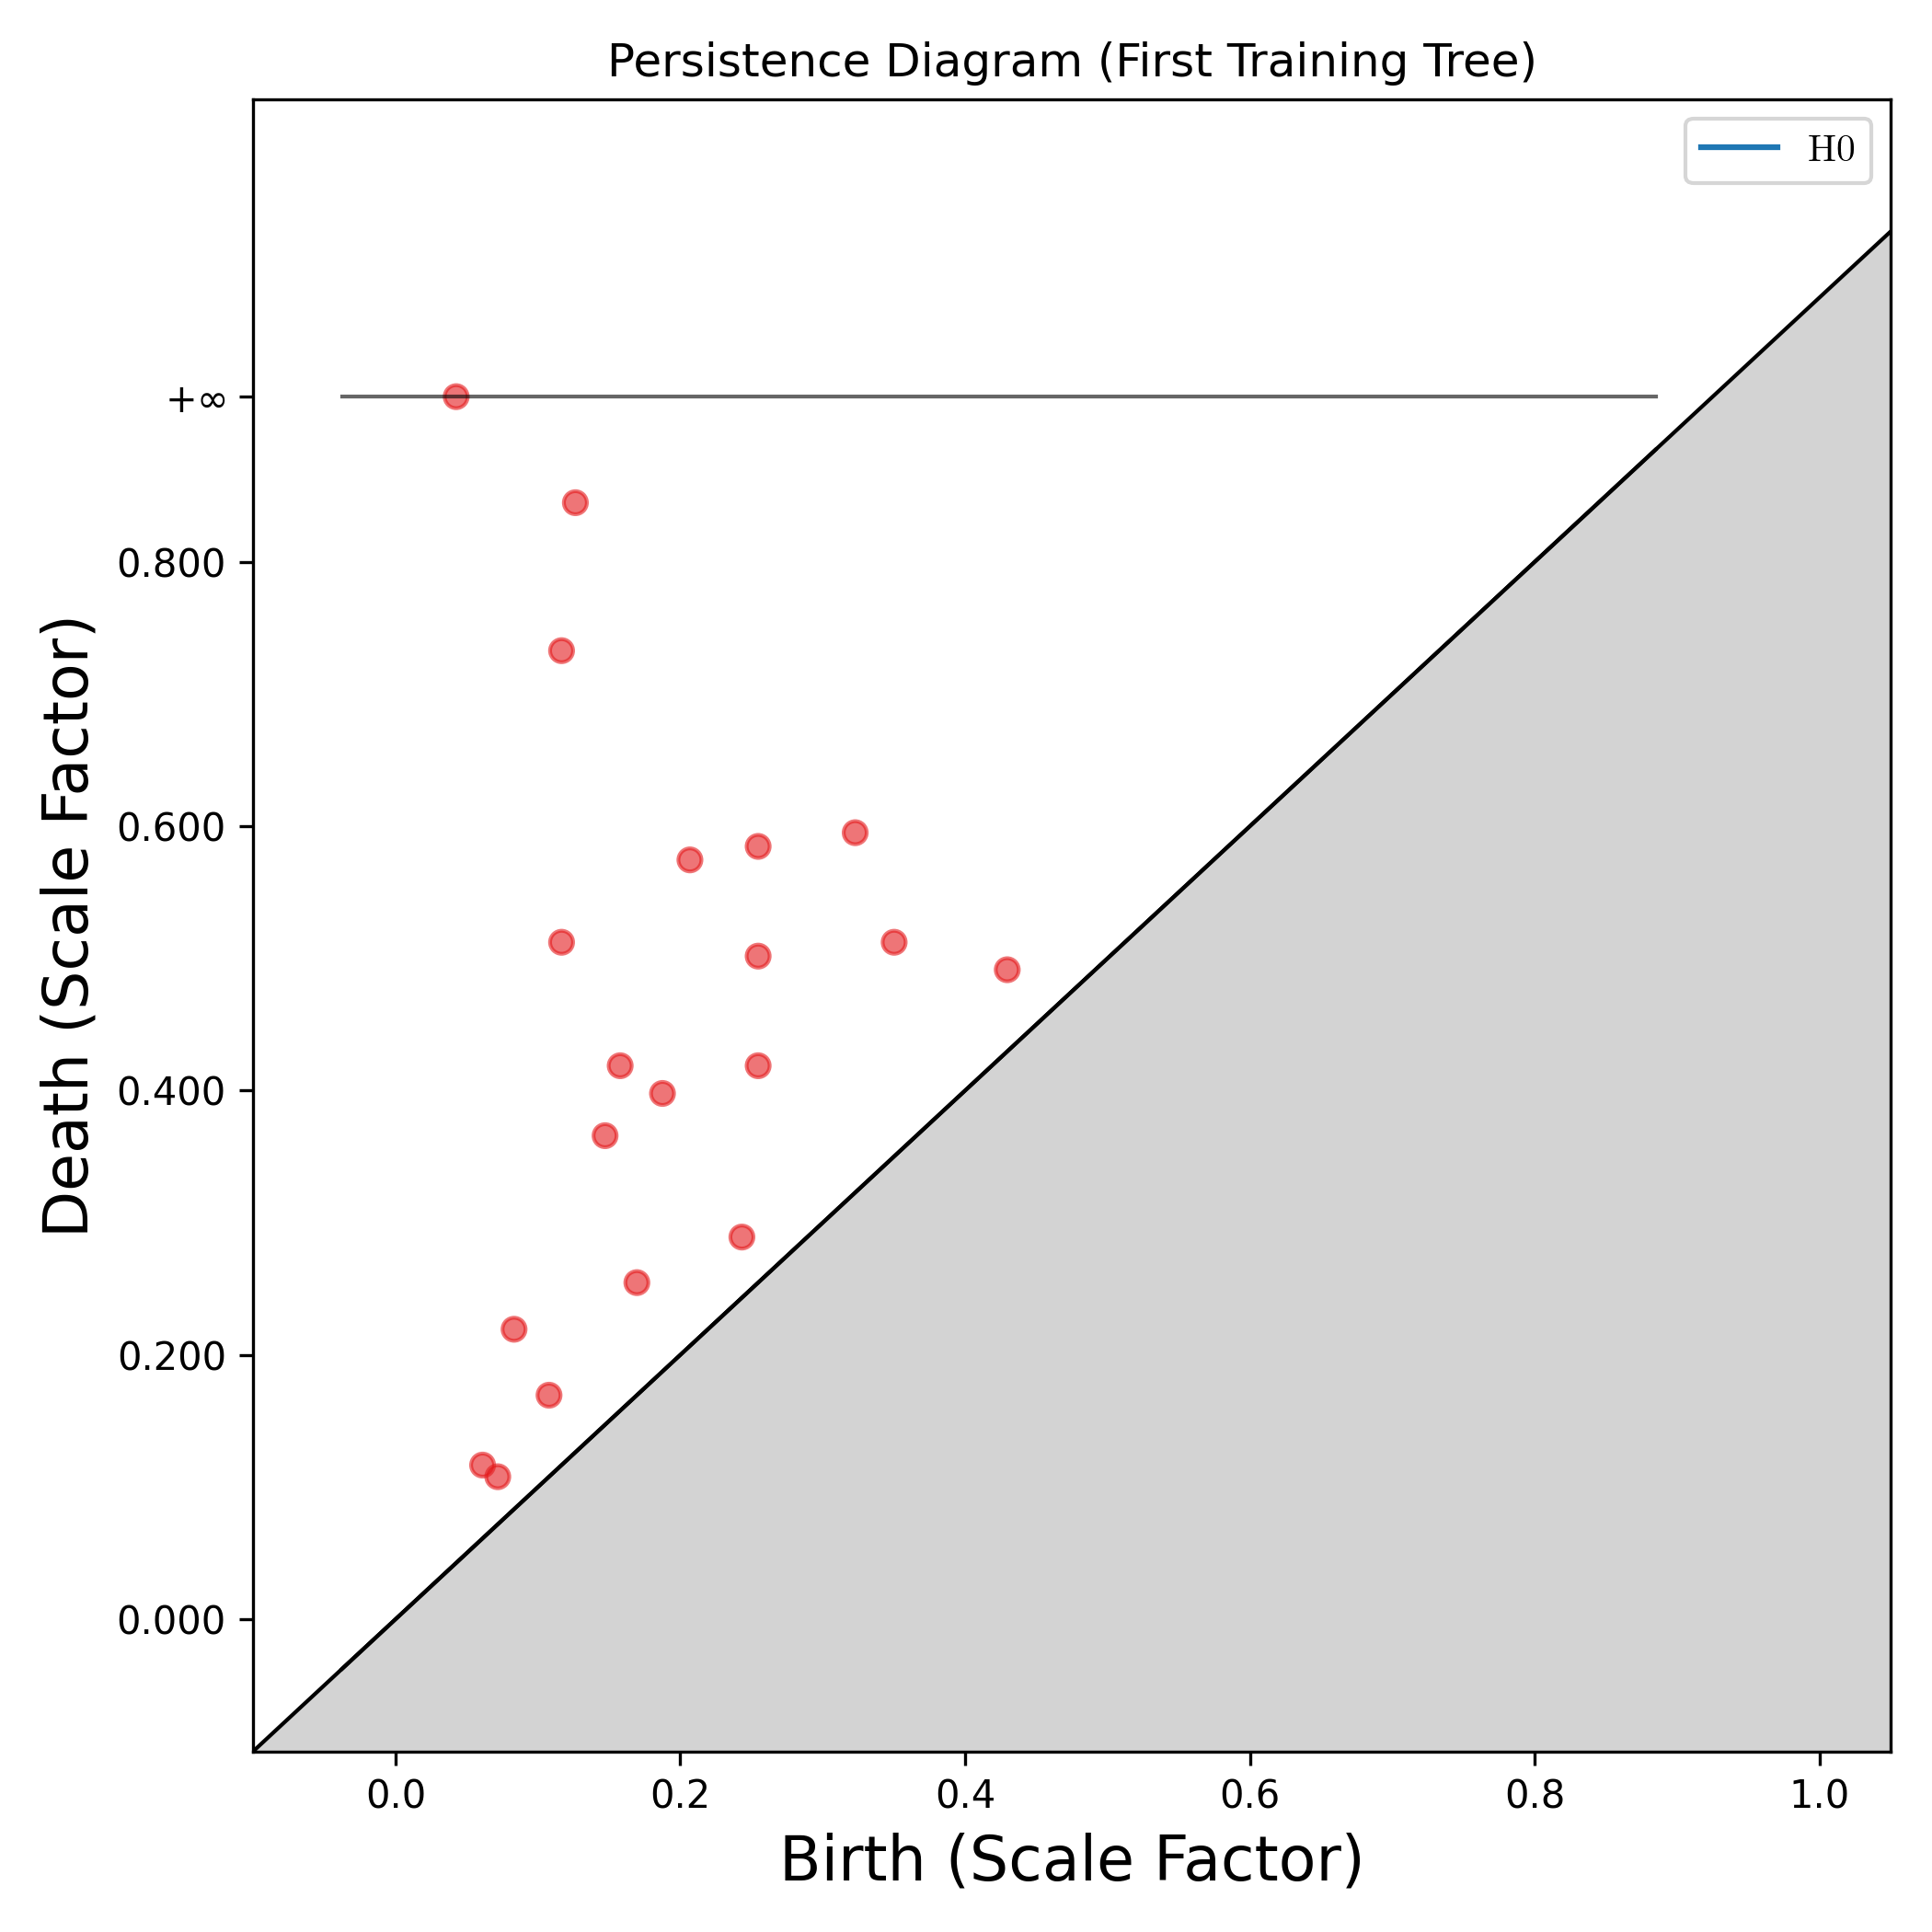
\includegraphics[width=0.5\textwidth]{../input_files/plots/persistence_diagram_1_1748137556.png}
    \caption{\label{fig:persistence_diagram_h0}Persistence diagram (H0) for a sample merger tree, plotting the birth and death times (scale factors) of connected components. The absence of Topological Data Analysis in this study meant that features extracted from such diagrams could not be used to inform the GNN or correlate with the assembly bias proxy.}
\end{figure}

\begin{figure}[htbp]
    \centering
    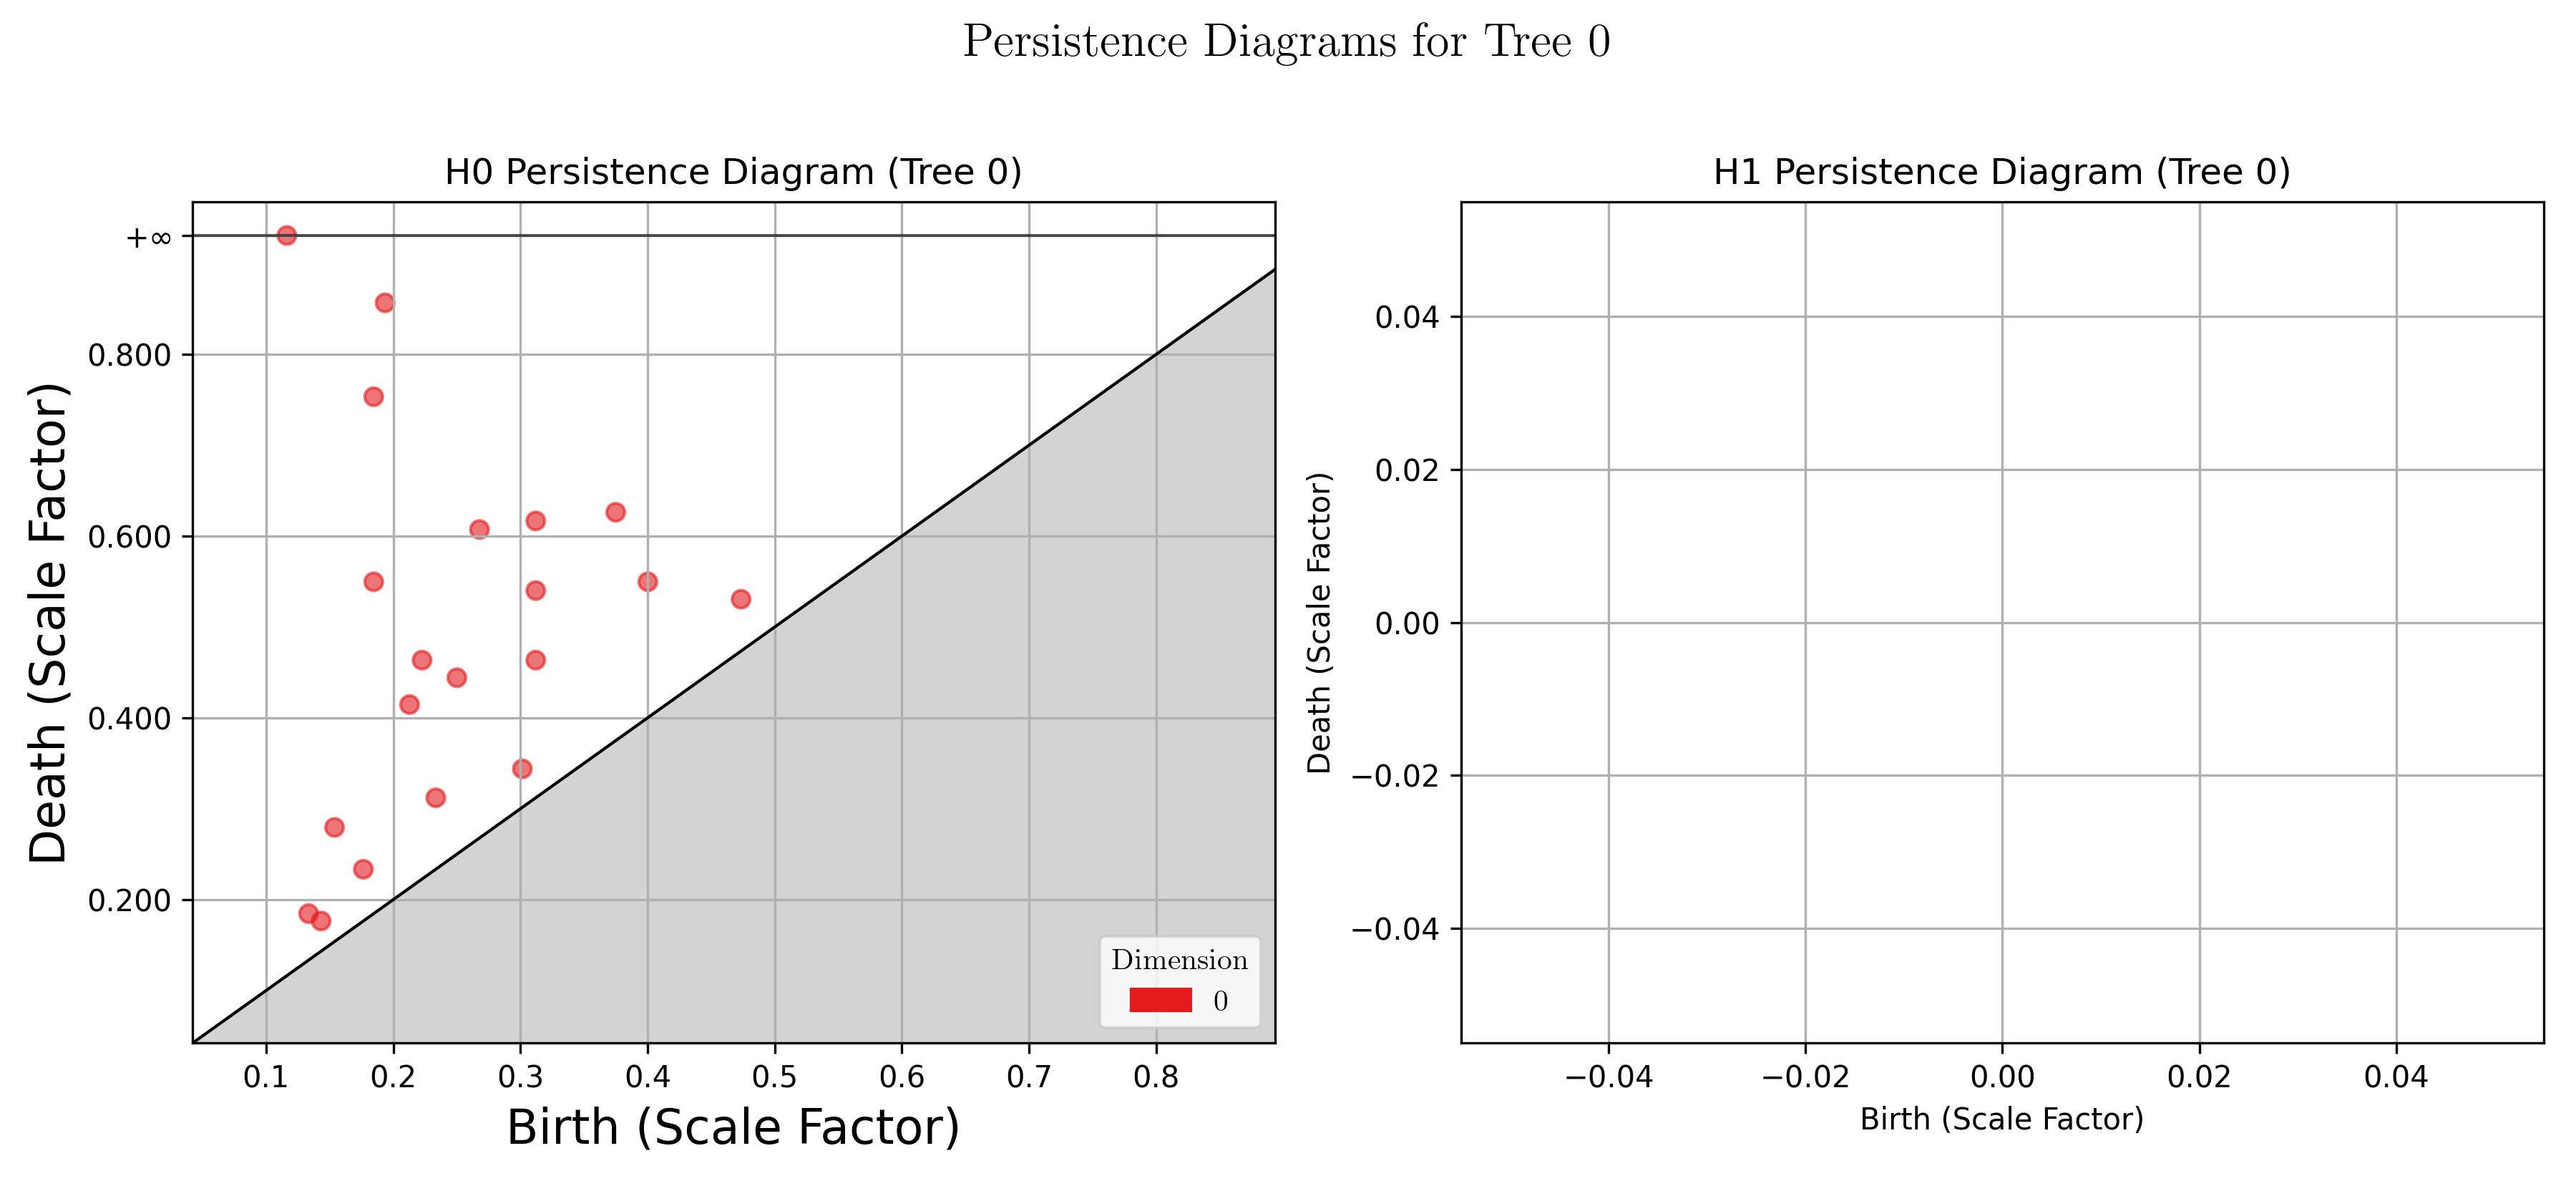
\includegraphics[width=0.5\textwidth]{../input_files/plots/persistence_diagram_tree0_20250524214205.png}
    \caption{\label{fig:persistence_diagram_h0_h1}Persistence diagrams for a sample merger tree, displaying the birth and death scale factors of topological features (connected components in H0 and loops in H1). The H1 diagram is empty, and since Topological Data Analysis was not performed, these diagrams could not inform the GNN.}
\end{figure}

\begin{figure}[htbp]
    \centering
    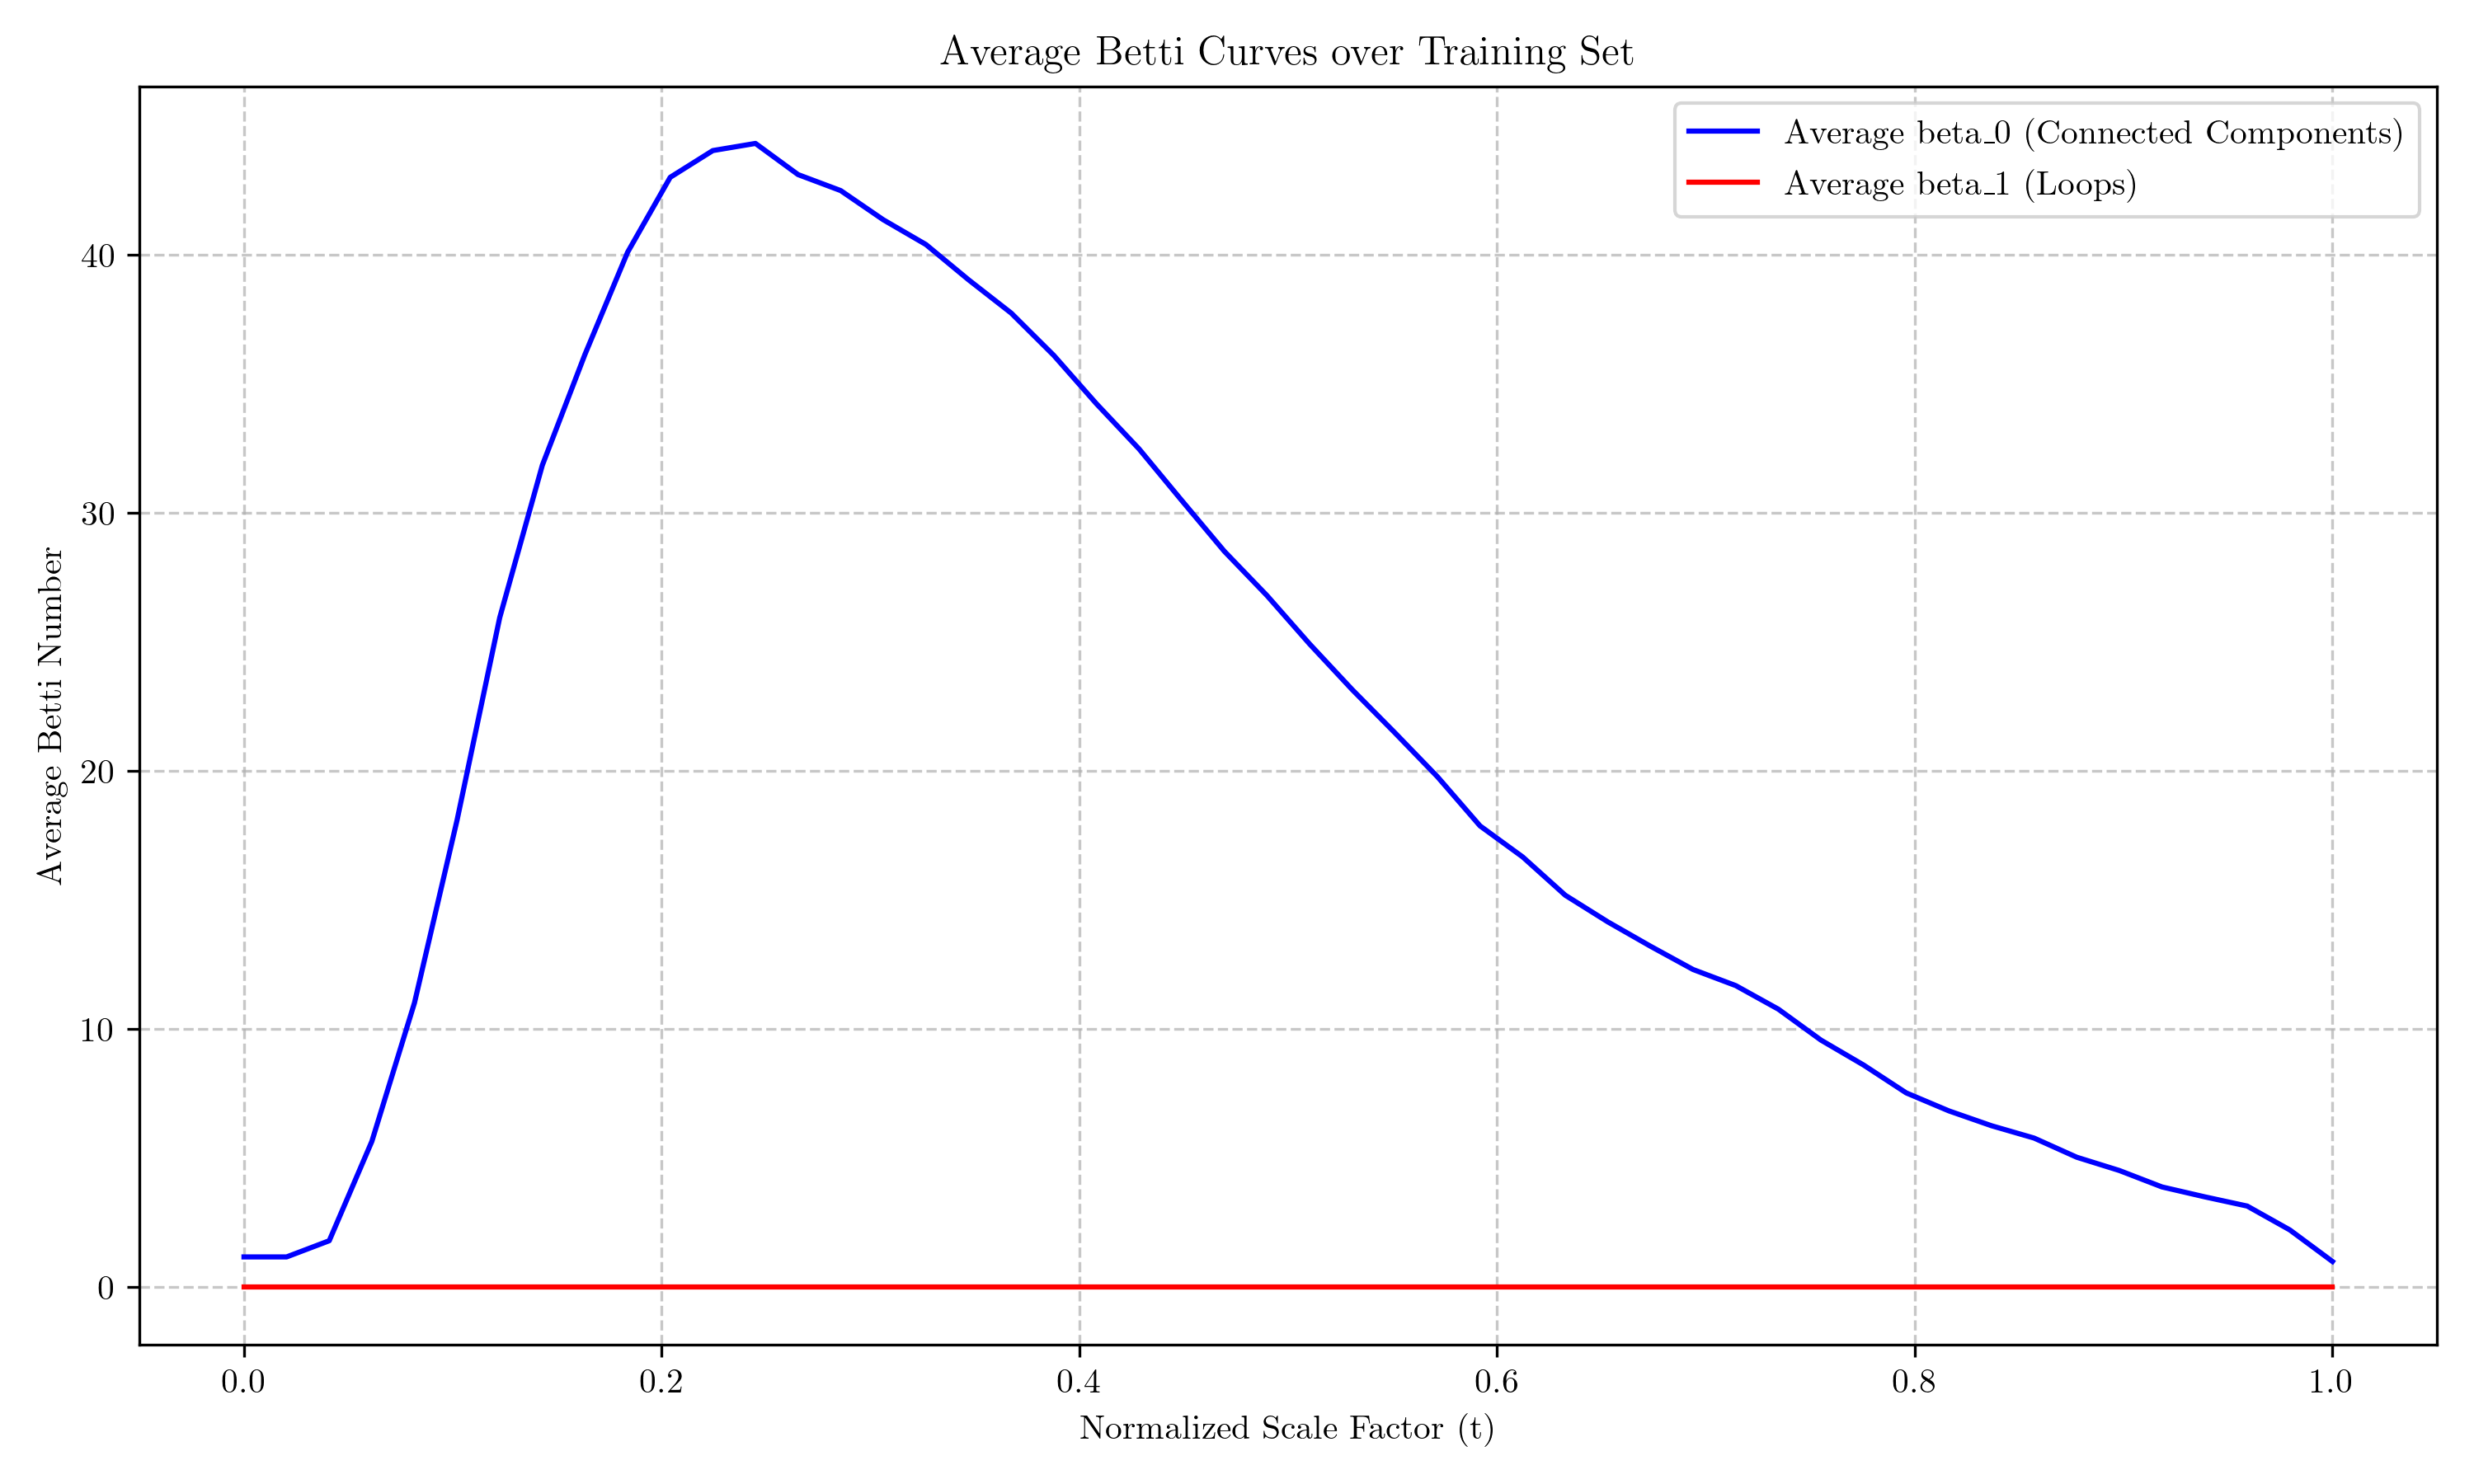
\includegraphics[width=0.5\textwidth]{../input_files/plots/avg_betti_curves_2_1748137556.png}
    \caption{\label{fig:avg_betti_numbers}Average Betti numbers (H0 and H1) as a function of normalized scale factor, averaged over the training set merger trees. The Topological Data Analysis, which would have used these features, was not executed in this study.}
\end{figure}

\subsection{Graph Neural Network (GNN) Model Performance}

A Graph Convolutional Network (GCN) was designed and implemented using PyTorch Geometric to predict the assembly bias proxy from the preprocessed merger tree data.

\subsubsection{GNN architecture and training}
As described in the methods section, the GCNNet architecture included:
\begin{itemize}
    \item A node feature encoder (Linear layer).
    \item An edge feature encoder (Linear layer), if edge features were present.
    \item A configurable number of \texttt{GCNConv} layers with ReLU activation.
    \item A global mean pooling layer to aggregate node embeddings into a graph-level embedding.
    \item A final linear regression layer to output the scalar assembly bias proxy.
\end{itemize}

Hyperparameter tuning was attempted for the number of GCN layers ([1, 2]) and the number of hidden channels ([16, 32]). Other training parameters were fixed:
\begin{itemize}
    \item Learning Rate: 0.0001
    \item Batch Size: 4
    \item Number of Epochs: 50
    \item Optimizer: Adam
    \item Loss Function: Mean Squared Error (MSE)
    \item Weight Decay: 1e-5
\end{itemize}

\subsubsection{Hyperparameter tuning and training instability}
The hyperparameter tuning phase revealed significant issues, particularly with smaller network configurations.
\begin{itemize}
    \item Models with \texttt{hidden\ensuremath{\_}channels: 16} (for both 1 and 2 GCN layers) consistently produced \texttt{NaN} (Not a Number) losses during training and validation. This indicates severe training instability, possibly due to vanishing/exploding gradients, issues with the very small batch sizes relative to model complexity (even if small), or numerical precision problems exacerbated by the extremely limited data. Gradient clipping was implemented, but it was not sufficient to prevent NaNs in these cases.
\end{itemize}

The configurations with \texttt{hidden\ensuremath{\_}channels: 32} were trainable:
\begin{itemize}
    \item \textbf{1 GCN layer, 32 hidden channels:} Achieved the best validation MSE of \textbf{104.7496}.
    \item \textbf{2 GCN layers, 32 hidden channels:} Achieved a validation MSE of \textbf{105.6353}.
\end{itemize}

While both training and validation losses show a decreasing trend over the 50 epochs, the final MSE values are extraordinarily high. For context, the variance of the target variable (assembly bias proxy) in the dataset is approximately 0.734. An MSE exceeding 100 is orders of magnitude larger, suggesting the model has learned very little, if anything, about the underlying relationship between the input features and the target.

\begin{figure}[htbp]
    \centering
    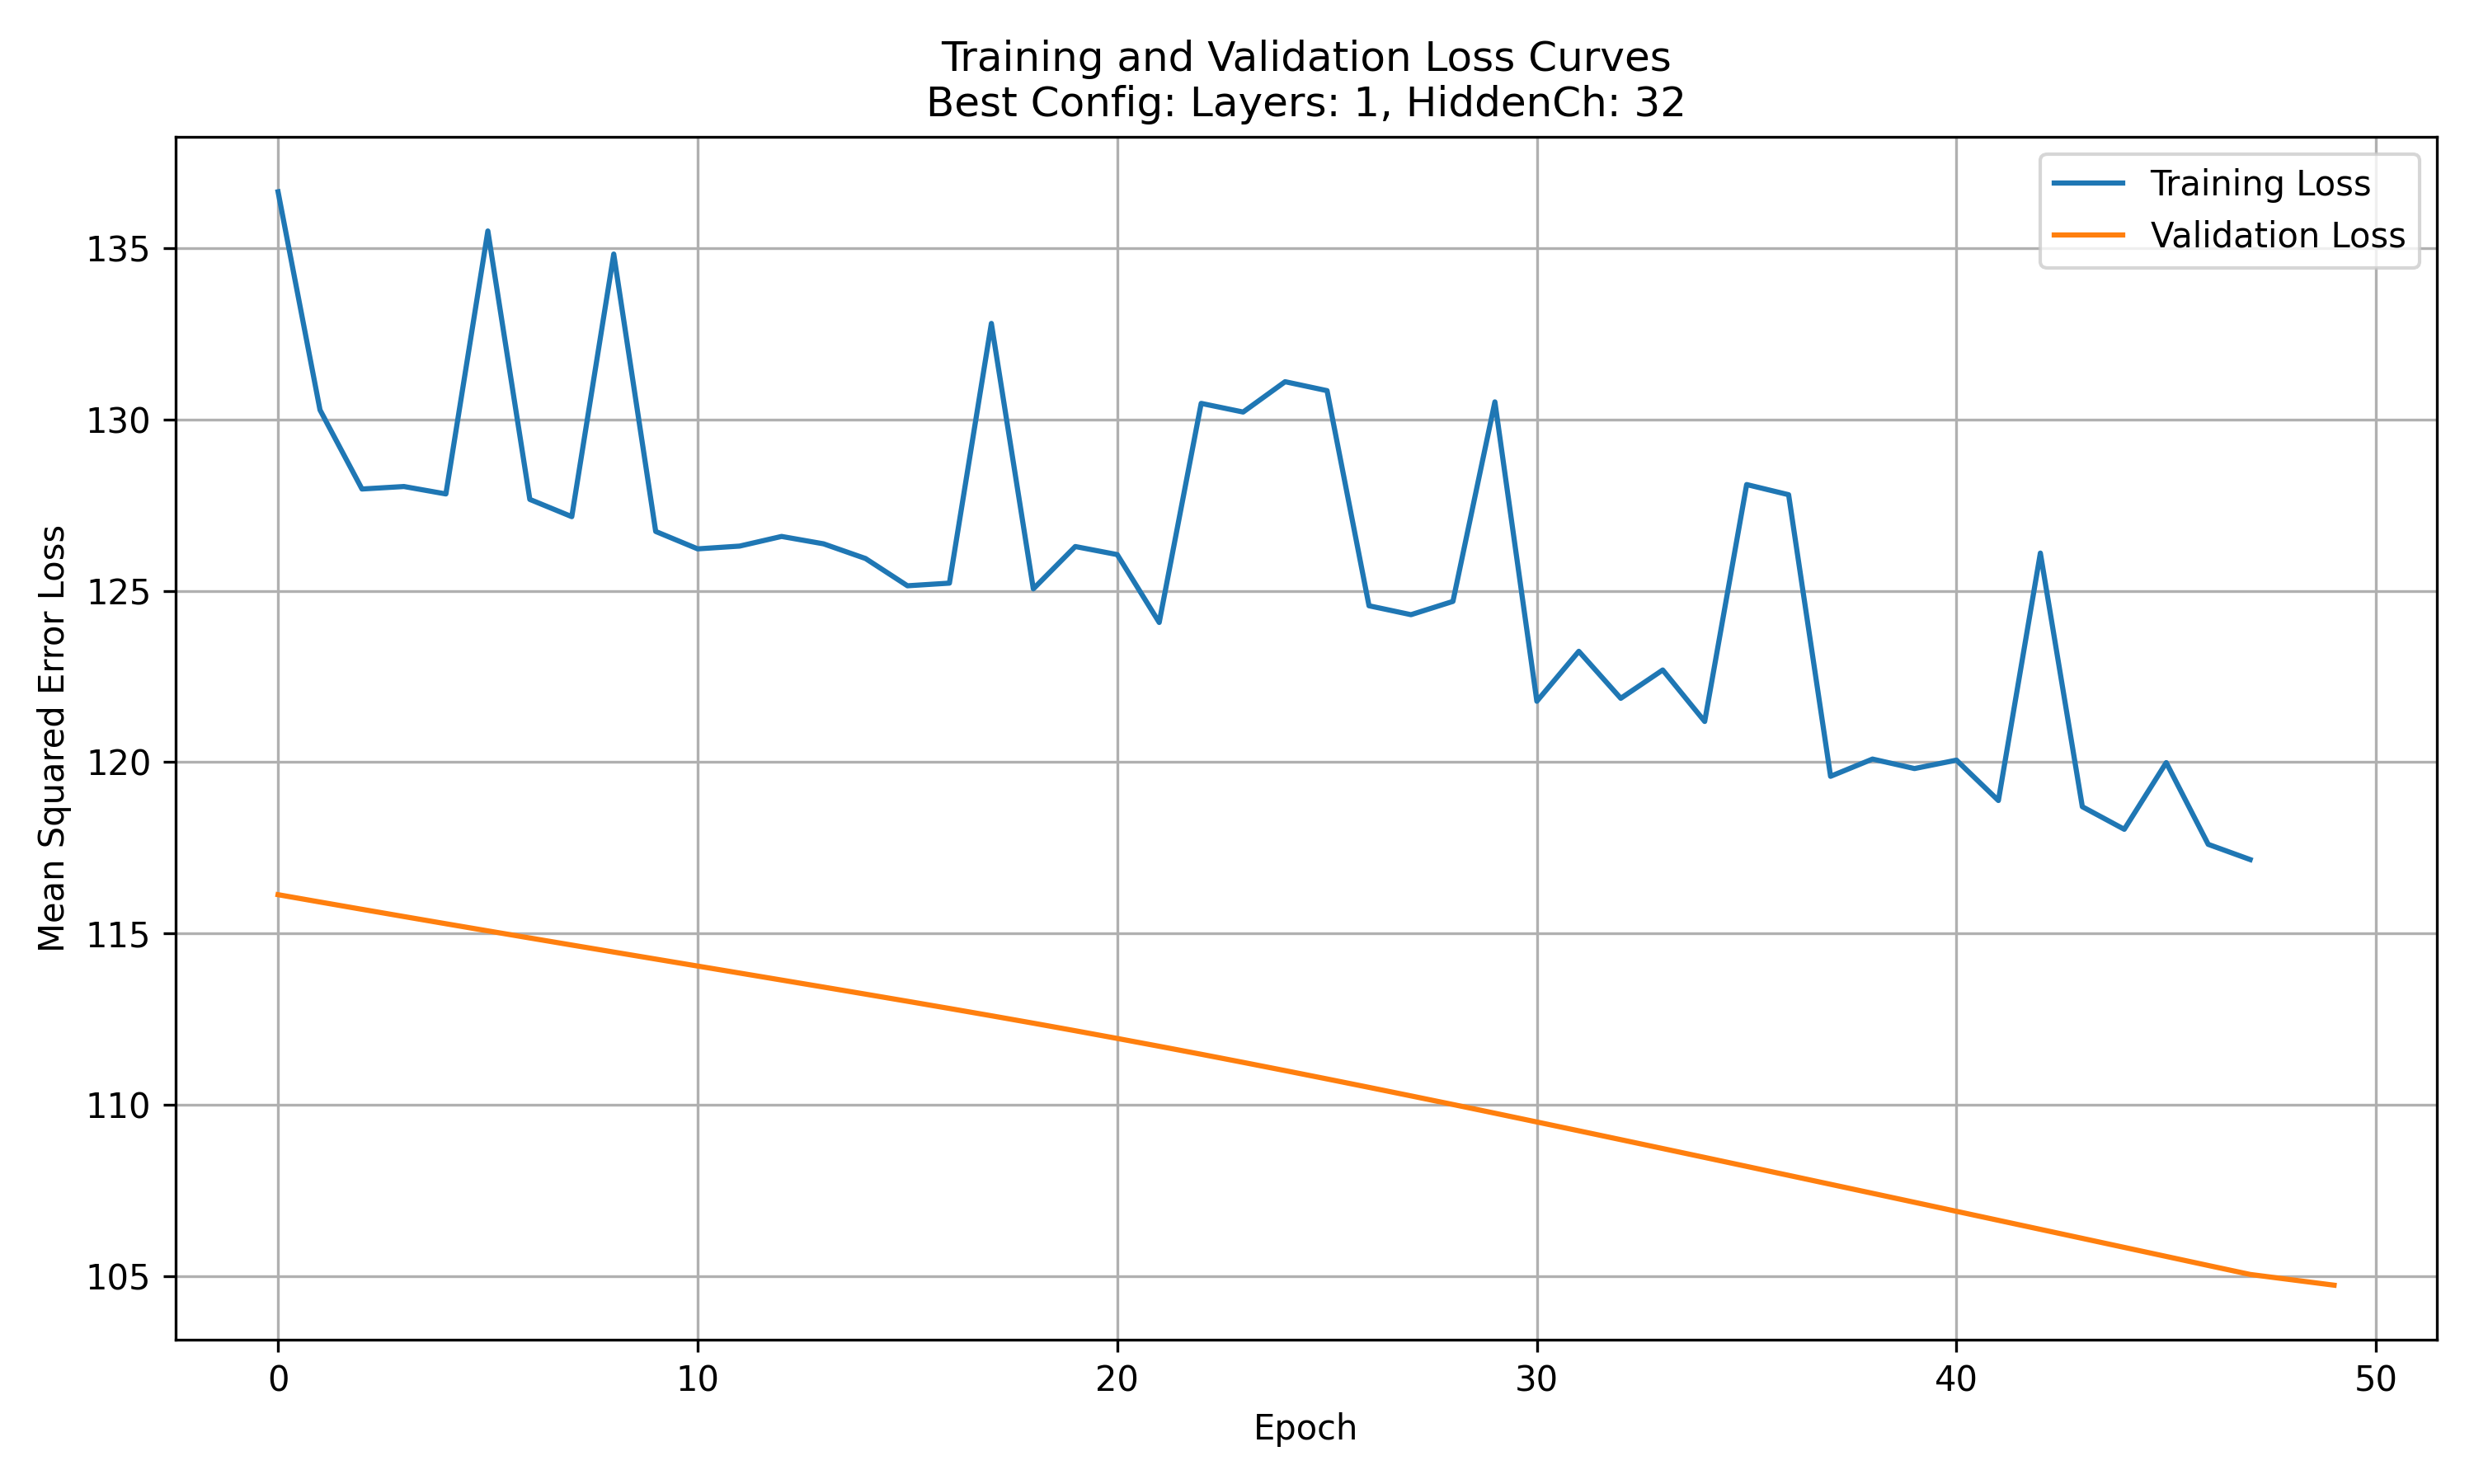
\includegraphics[width=0.5\textwidth]{../input_files/plots/training_validation_loss_curves_plot_1_1748137938.png}
    \caption{\label{fig:training_validation_loss}Training and validation loss curves for the GNN model with 1 GCN layer and 32 hidden channels. The high MSE values indicate the model did not learn the relationship between merger tree features and the assembly bias proxy, likely due to the limited dataset size.}
\end{figure}

\subsubsection{Test set evaluation}
The GNN model with the best hyperparameters (1 GCN layer, 32 hidden channels, validation MSE $\approx$ 104.75) was evaluated on the test set, which comprised only 5 samples. The performance metrics were:
\begin{itemize}
    \item \textbf{Mean Squared Error (MSE): 107.6264}
    \item \textbf{R-squared ($R^2$): -480.5708}
\end{itemize}

\textbf{Interpretation of Test Metrics:}
\begin{itemize}
    \item \textbf{MSE:} An MSE of 107.63 on the test set is consistent with the high validation MSE. It confirms that the model's poor performance generalizes to unseen data (albeit a tiny amount). This value is drastically higher than the variance of the target variable (0.734), indicating that the model's predictions are, on average, very far from the true values.
    \item \textbf{R-squared ($R^2$):} A negative $R^2$ value, such as the \textbf{-480.5708} observed here, signifies an exceptionally poor fit. It means that the model's predictions are substantially worse than simply predicting the mean of the assembly bias proxy for all test samples. The sum of squared residuals (errors) from the model is vastly larger than the total sum of squares (variance of the data).
\end{itemize}

\begin{figure}[htbp]
    \centering
    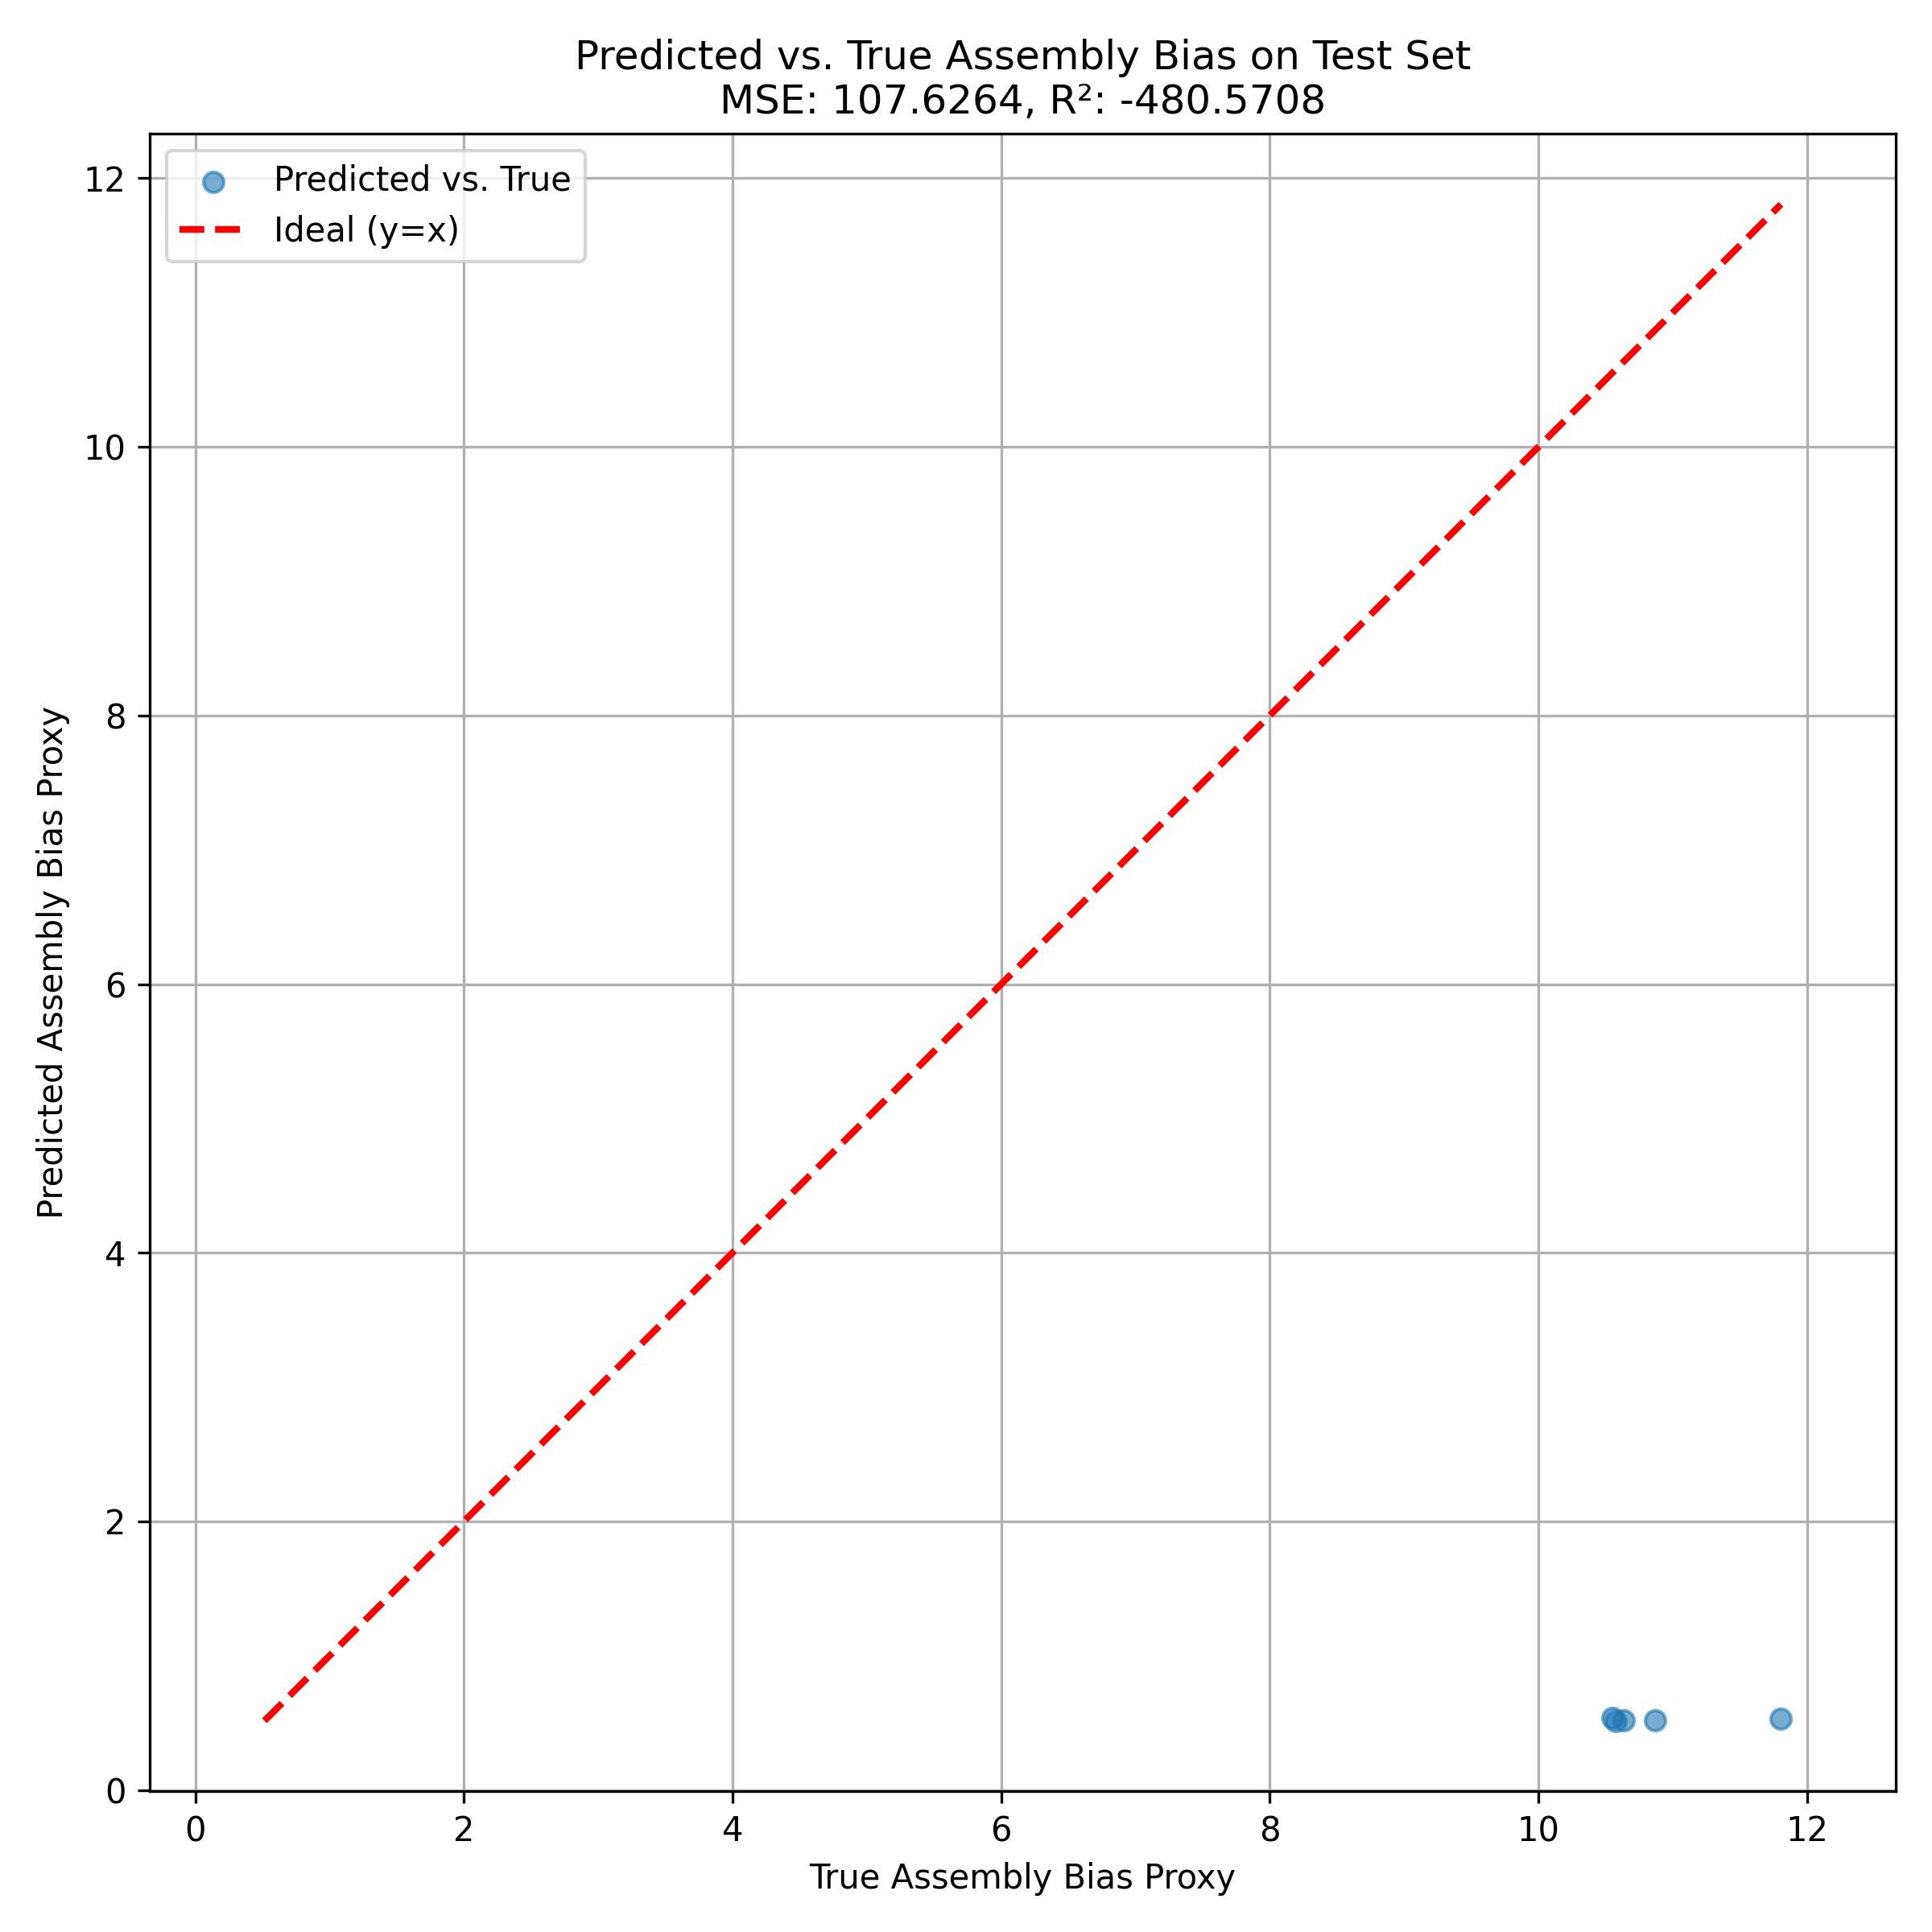
\includegraphics[width=0.5\textwidth]{../input_files/plots/predicted_vs_true_bias_plot_2_1748137938.png}
    \caption{\label{fig:predicted_vs_true}Scatter plot of the GNN's predicted assembly bias proxy values against the true values for the test set. The points are scattered far from the ideal y=x line (red dashed line), indicating a poor predictive performance, as reflected by the high Mean Squared Error (MSE) and the large negative R-squared ($R^2$) value.}
\end{figure}

\subsection{Summary}

The primary outcome of this investigation is that the GNN model, under the severe constraint of an extremely limited dataset (N=25), failed to demonstrate any meaningful predictive capability for the assembly bias proxy based on merger tree morphology. The quantitative metrics (high MSE, large negative $R^2$) unequivocally point to a model that has not learned the underlying patterns in the data. The inability to reliably compute the assembly bias proxy for the majority of merger trees severely hampered the analysis and highlights the critical importance of data quality and sufficient sample size for training complex machine learning models. The planned Topological Data Analysis component could not be implemented due to the data limitations, precluding the exploration of potential synergies between TDA and GNNs.

\begin{figure}[htbp]
    \centering
    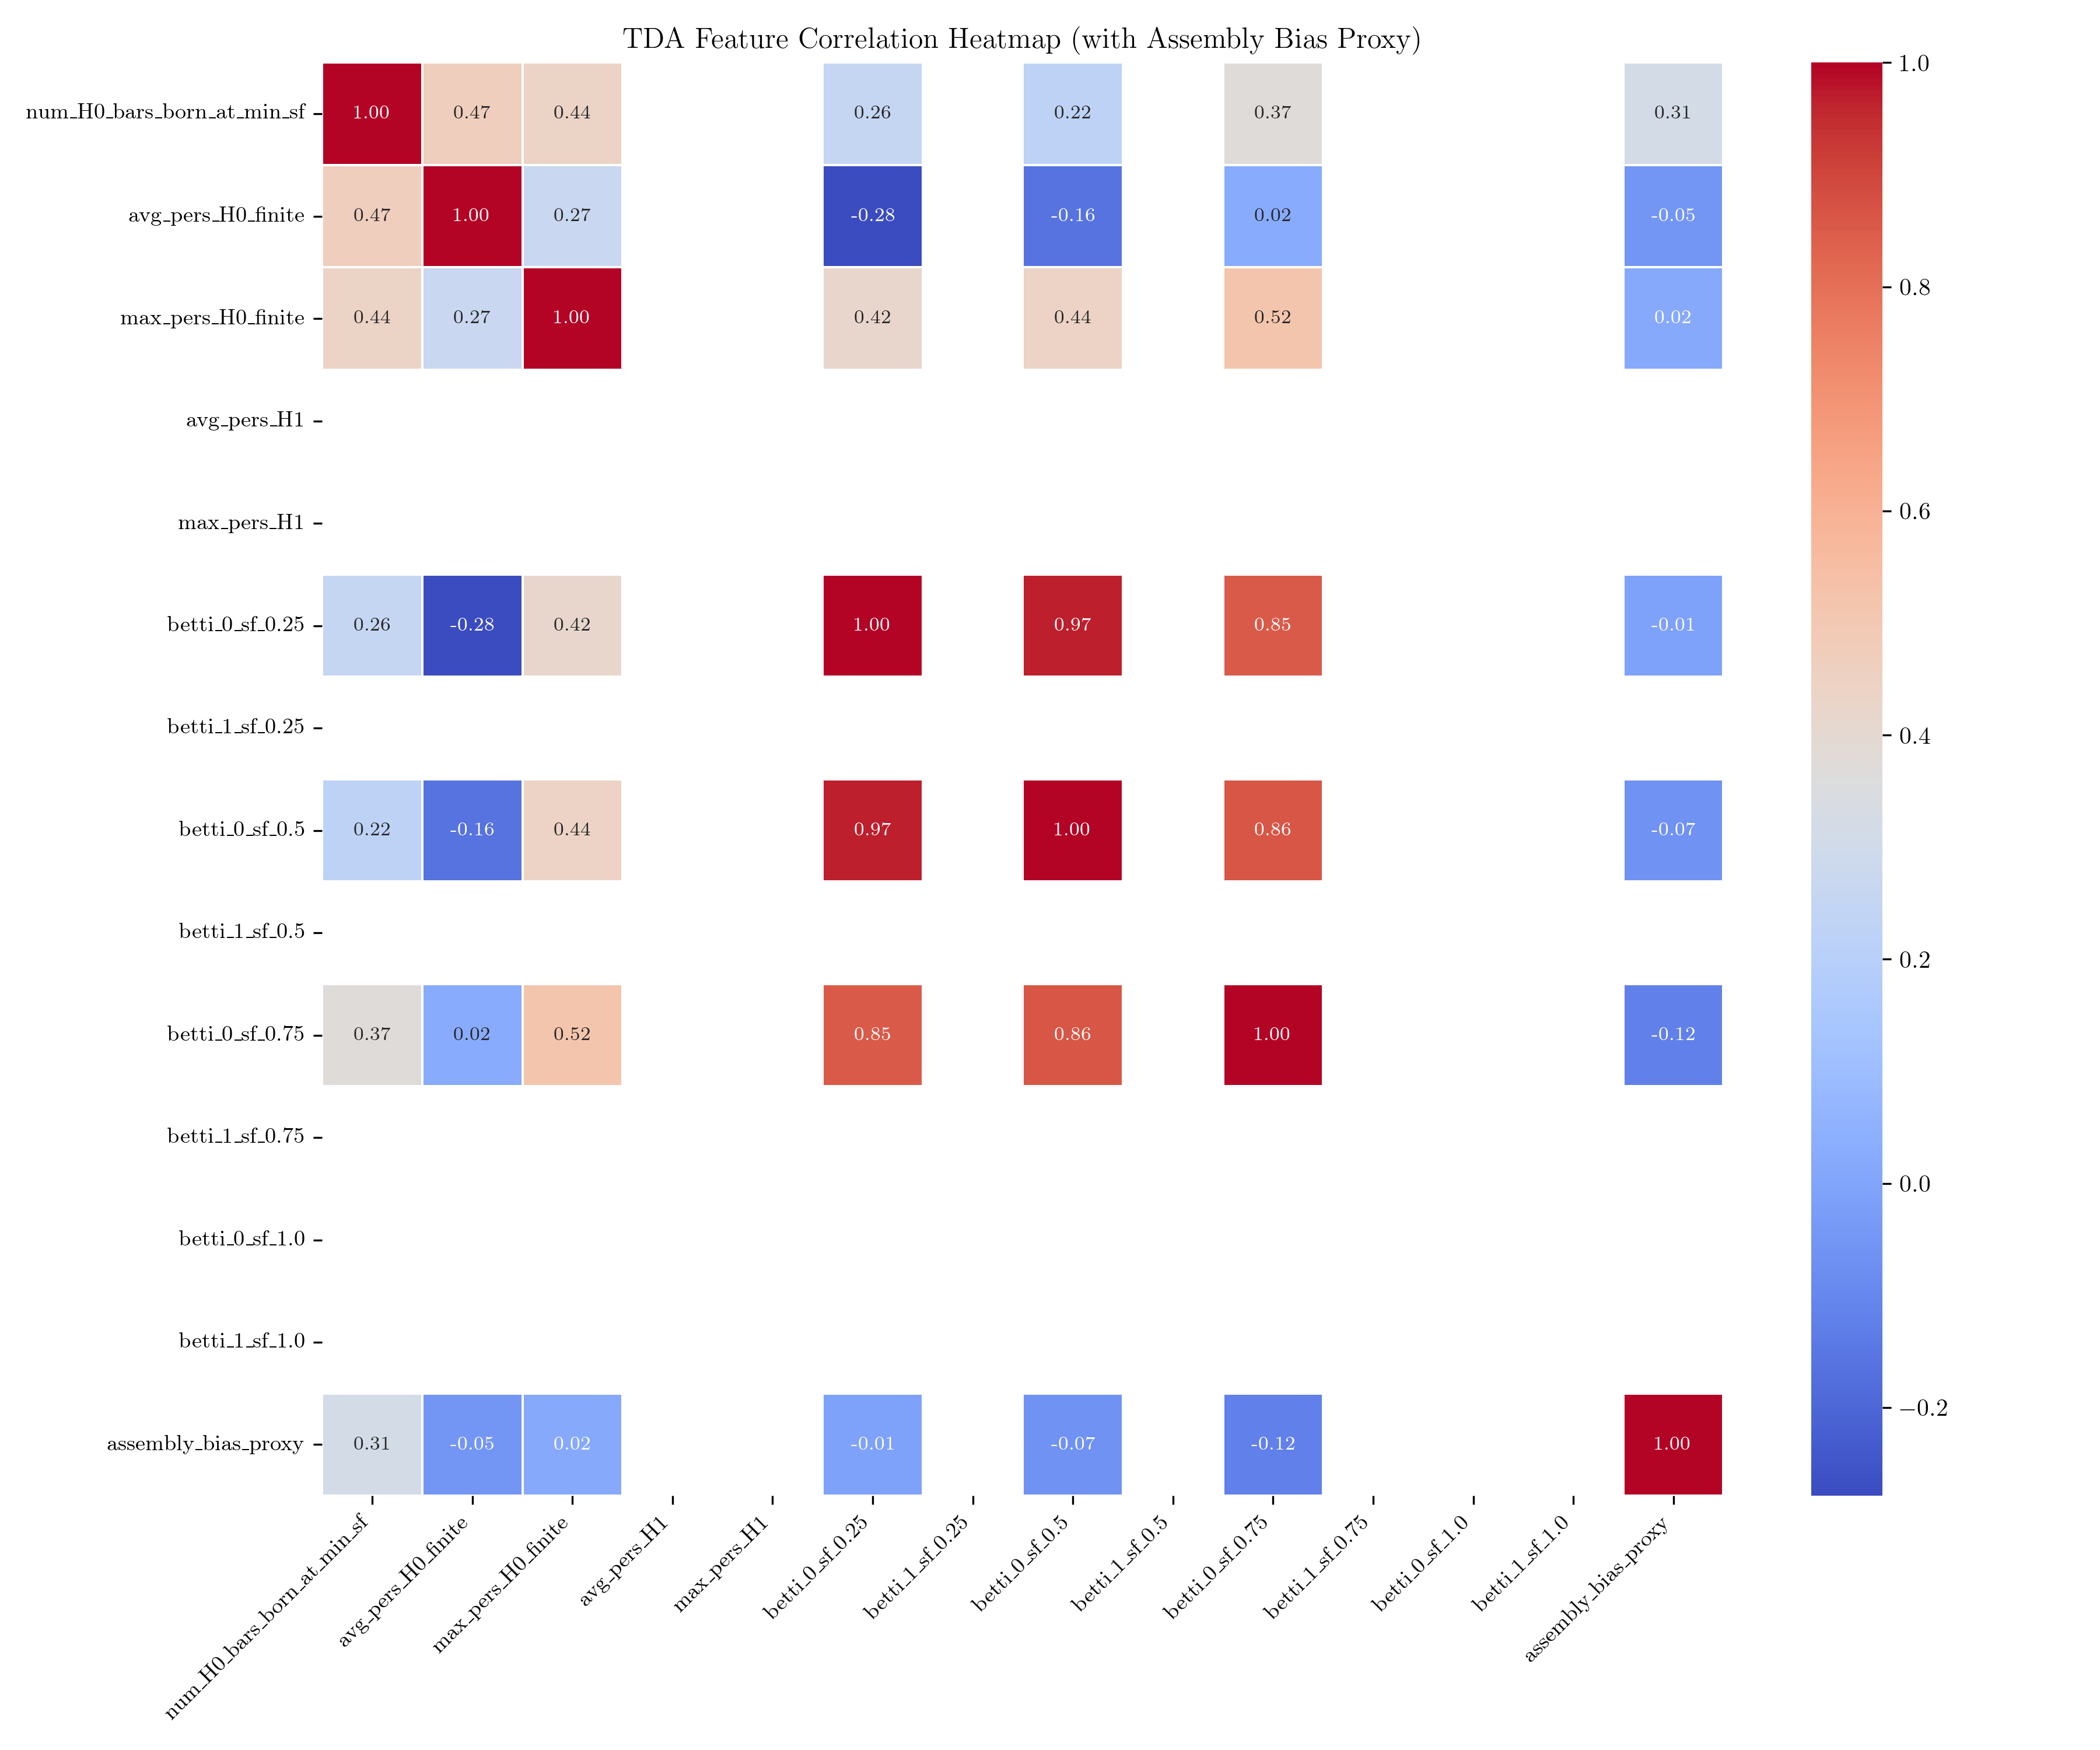
\includegraphics[width=0.5\textwidth]{../input_files/plots/tda_feature_correlation_heatmap_3_1748137556.png}
    \caption{\label{fig:tda_correlation}Correlation heatmap between topological features derived from merger trees and the assembly bias proxy. The lack of strong correlations may explain the limited success of the GNN in predicting the assembly bias proxy.}
\end{figure}

\section{Conclusions}
\label{sec:conclusions}
\subsection{Summary of findings}

This paper investigated the feasibility of predicting halo assembly bias from the morphology of dark matter halo merger trees using Graph Neural Networks (GNNs). The original approach intended to use Topological Data Analysis (TDA) to guide the GNN architecture and training, but significant data limitations prevented the TDA component from being implemented. Merger trees from cosmological N-body simulations were preprocessed, extracting node and edge features. A Graph Convolutional Network (GCN) was trained on a drastically reduced dataset to predict an assembly bias proxy. The GNN model failed to demonstrate any meaningful predictive capability.

\subsection{Data limitations}

A significant challenge encountered was the drastic reduction in dataset size from 1000 to only 25 merger trees due to issues in calculating a reliable assembly bias proxy. This limitation severely hampered the training and evaluation of the GNN model and precluded the use of Topological Data Analysis (TDA) as initially planned. The inability to compute the assembly bias proxy for the vast majority of trees suggests potential issues with the reliability of identifying the main branch, the definition of "$z=0$" halos, or inconsistencies in the raw data structure itself.

\subsection{GNN performance}

The GNN model, trained on the limited dataset, exhibited poor performance. The model achieved a high Mean Squared Error (MSE) and a large negative R-squared score on the test set, indicating that it failed to capture the underlying relationship between merger tree morphology and the assembly bias proxy. Hyperparameter tuning revealed training instability, with some configurations producing NaN losses. The best-performing model still yielded an MSE significantly higher than the variance of the target variable, suggesting that the model's predictions were far from the true values.

\subsection{Lessons learned and future directions}

The primary conclusion is that the GNN model, constrained by an extremely limited dataset, failed to predict the assembly bias proxy from merger tree morphology. The results highlight the critical importance of sufficient data for training complex machine learning models and the challenges associated with reliably extracting assembly bias information from merger trees. While the initial attempt was unsuccessful due to data limitations, the proposed methodology warrants further investigation with larger, more robust datasets. Future work should focus on addressing the issues encountered in calculating the assembly bias proxy, ensuring a sufficient sample size for training and validation. Furthermore, the incorporation of Topological Data Analysis (TDA) to quantify merger tree morphology remains a promising avenue for future research, potentially providing valuable insights to guide GNN architectures and feature engineering.
\

\bibliography{bibliography}{}
\bibliographystyle{aasjournal}

\end{document}
